\section{Background and Related Work}
\label{sec:background}

Several server consolidation solutions are available in the literature. Their main framework consists in monitoring the virtual servers, predicting their future resource consumption, and deciding which action should be taken to optimise a given metric. Number of physical servers, number of virtual machine migrations, energy consumption, and server availability are examples of optimisation metrics. The solutions vary in aspects such as frequency when actions take place, whether they are proactive by using a prediction method or reactive by verifying resource consumption values, and costs for resizing and moving virtual machines.

One server consolidation solution is proposed by Khanna et al.~\cite{khanna2006application}, which consists in a dynamic management algorithm that is triggered when a physical server becomes overloaded or underloaded. The main goals of their algorithm are to: i) guarantee that SLAs are not violated; ii) minimise migration cost; iii) optimise the residual capacity of the system; and iv) minimise the number of physical servers used. Bobroff et al.~\cite{bobroff2007dynamic} proposed and evaluated a dynamic server consolidation algorithm to reduce the amount of required capacity and the rate of SLA violations. The algorithm uses historical data to forecast future demand and relies on periodic executions to minimise the number of physical servers to support the virtual machines.

Speitkamp and Bichler~\cite{bichler2006capacity, speitkamp2010mathematical} described linear programming formulations for the static and dynamic server consolidation problems. They also designed extension constraints for limiting the number of virtual machines in a physical server, guaranteeing that some virtual machines are assigned to different physical servers, mapping virtual machines to a specific set of physical servers that contain some unique attribute, and limiting the total number of migrations for dynamic consolidation. In addition, they proposed an LP-relaxation based heuristic for minimising the cost of solving the linear programming formulations. Mehta and Neogi~\cite{mehta2008recon} introduced the ReCon tool, which aims at recommending dynamic server consolidation in multi-cluster data centres. ReCon considers static and dynamic costs of physical servers, the costs of VM migration, and the historical resource consumption data from the existing environment in order to provide an optimal dynamic plan of VMs to physical server mapping over time. Similarly, Verma et al.~\cite{verma2008pmapper} developed the pMapper architecture and a set of server consolidation algorithms for heterogeneous virtualized resources. The algorithms take into account power and migration costs and the performance benefit when consolidating applications into physical servers.

Wood et al.~\cite{wood2009sandpiper} developed the Sandpiper system for monitoring and detecting hotspots, and remapping/reconfiguring VMs whenever necessary. In order to choose which VMs to migrate, Sandpiper sorts them using a volume-to-size ratio (VSR), which is a metric based on CPU, network, and memory loads. Sandpiper tries to migrate the most loaded VM from an overloaded physical server to one with sufficient spare capacity.

Most of these solutions rely on monitoring and predicting future load. Server
consolidation strategies may not be able to produce optimised actions if future
load prediction is not accurate. For instance, Figure~\ref{fig:background} illustrates a scenario with one physical machine that hosts two virtual machines. One physical machine is off. The prediction system detects that one of the virtual machines will require more computing power. As both virtual machines do not fit into the same physical machine, the management system switches on the second physical machine. If the virtual machine really requires more resources, it is moved to the second physical machine. If the prediction was not correct and the virtual machine’s resource demand did not change, it remains on the first physical machine, thus wasting energy as the second physical machine was switched on. Given this scenario, the question investigated in this paper is therefore “What is the impact of load prediction accuracy on existing server consolidation solutions?”.

\begin{figure*}[th]
\centerline{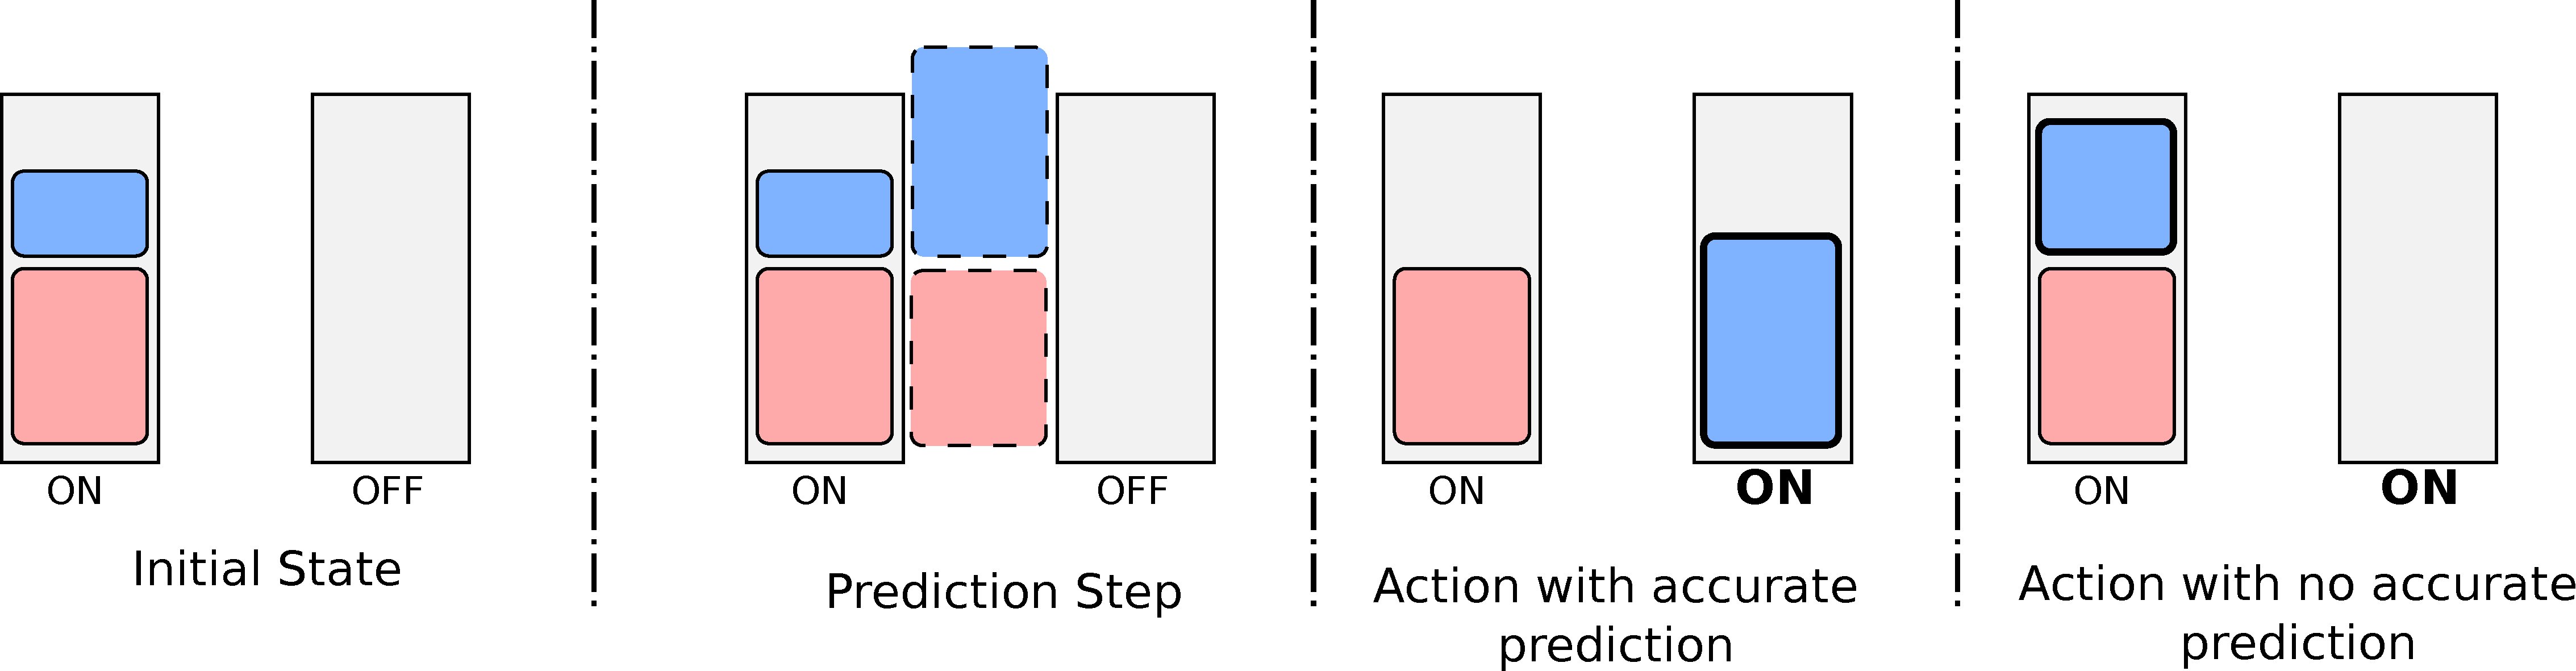
\includegraphics[width=1.00\textwidth]{background.pdf}}
\vspace{-2mm}
\caption{Illustrative scenario where one physical machine hosts two virtual machines. One physical machine is off. If the prediction is correct, the second physical machine is switched on and the virtual machine is moved to it. If the prediction is not correct, the second machine is switched on but no virtual machine is moved to it, thus wasting energy.}
\vspace{-1mm}
\label{fig:background}
\end{figure*}

\cite{netto2011use}
